%!TEX root = ../thesis.tex

\chapter{The Local Rossby Number}
\label{chap:rol}
One factor which makes dynamos difficult to understand is the large number of control parameters that are required to specify a solution to the governing equations. This is particularly troubling because the properties of a dynamo is dependent on the values of these control parameters. Unfortunately for numerical reasons dynamo models must be run in a parameter regime for which none of the control parameters is realistic.

\citet{christensen06scaling} developed a scaling law concerning planetary dynamos which has proved to be useful in the prediction of the bulk properties of a dynamo as a function of its control parameters. The Rossby number is normally defined as the ratio of the inertial force to the Coriolis force, from equation \ref{eq:navierstokesgeneralcorlor} this is
\begin{align*}
Ro&=\frac{\rho \mbf{u}\cdot\nabla\mbf{u}}{2\rho\mbf{\Omega}\times\mbf{u}}\\
&\approx\frac{U}{2\Omega L}\\
&\approx\frac{U}{\Omega r_o}.
\end{align*}
\citet{christensen06scaling} noted that while the inertial term depends on the length scale of the flow, the Coriolis term does not. They posited that a better measure of the role rotation plays in a given flow may be a Rossby number which depends on the characteristic length scale of the flow, rather than the characteristic length scale of the container. They defined this length scale as
\begin{equation}
\label{eq:rollength}
\bar{\ell}_{u}=\frac{4Ro_m^2}{\left(1-r_{io}\right)^2}\frac{\sum l\left\langle\mbf{u}_{l}\cdot\mbf{u}_{l}\right\rangle}{2E_{kin}}
\end{equation}
Where $E_{kin}$ is the kinetic energy, defined as
\begin{equation}
E_{kin}=\frac{4 Ro_m^2}{\left(1-r_{io}\right)^{5}}\frac{1}{2}\int_{V}\left(\mbf{u}\cdot\mbf{u}\right)dV
\end{equation}
using the non-dimensionalisation of \citet{kuangandbloxham1999}. Combining these we get
\begin{equation}
\bar{\ell}_{u}=\left(1-r_{io}\right)^{3}\frac{\sum l\left\langle\mbf{u}_{l}\cdot\mbf{u}_{l}\right\rangle}{\int_{V}\left(\mbf{u}\cdot\mbf{u}\right)dV}.
\end{equation}
Since the mean radius to a point inside the shell is of order one, they set the half wavelength of the flow to $\pi/\ell_u$ giving a local Rossby number of 
\begin{equation}
\label{eq:rol}
Ro_{l}=Ro\frac{\bar{\ell}_{u}}{\pi}.
\end{equation}

\citet{christensen06scaling} then noted that the dipole dominance of the poloidal magnetic field depended strongly on the local Rossby number. They showed that dynamo models which had $Ro_{l}\leq 0.12$ had magnetic fields that were predominantly dipolar, while models with $Ro_{l}>0.12$ generated multipolar magnetic fields. This sharp transition is clear if the dipole dominance of the observable magnetic field ($f_{dip}$) is plotted against the local Rossby number (figure \ref{fig:rolfdip}). Using angle brackets to denote a time average, $f_{dip}$ is defined as
\begin{equation}
f_{dip}=\left\langle\frac{ \int_S \sqrt{\mbf{B}_{l=1}\cdot\mbf{B}_{l=1}} }{\sum_{l=1}^{12} \mbf{B}_{l}\cdot\mbf{B}_{l}}\biggr\rvert_{r=r_{o}}\right\rangle
\end{equation}
which is the time average ratio of the r.m.s. amplitude of the dipole field to the r.m.s. amplitude of the field in the first 12 degrees.
\begin{figure}
	\centering
	\noindent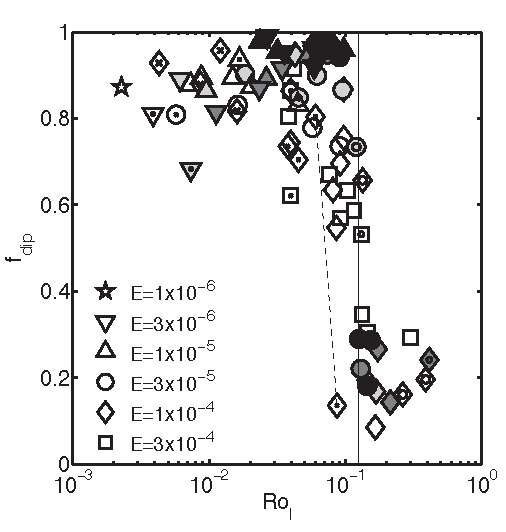
\includegraphics[width=.5\linewidth]{Appendix2/figures/fdip.pdf}
	\caption{The dipole dominance ($f_{dip}$) of the observable magnetic field as a function of the local Rossby number. Here $f_{dip}$ is defined as the time average ratio of the r.m.s. amplitude of the dipole field to the r.m.s. amplitude of the field in the first 12 degrees. The Ekman numbers here are in the variables of \citet{christensen06scaling}, they can be converted to the Ekman numbers in this work by multiplying them by a factor of $0.21125$. This figure is reproduced from \citet{christensen06scaling} where it is figure 3.}
	\label{fig:rolfdip}
\end{figure}

Once the local Rossby number is defined, a natural extension is to apply it to the planets of our solar system. The definition of equation \ref{eq:rol} requires a knowledge the characteristic fluid velocity and scale in the fluid outer core. This is very unconstrained for even the Earth, and less well constrained for other planets of our solar system. An alternative approach is to construct scaling laws which relate the control parameters of the dynamo to the local Rossby number. The control parameters depend on the physical properties of the planet (e.g. diffusivities, rotation rates etc.) which are known more accurately than the dynamical properties (i.e. the scale of convection).

Several studies have constructed scaling laws which relate the dynamo control parameters to the local Rossby number \citep{christensen06scaling,OlsonandChristensen2006,aubert2009}. The most general is from \citet{aubert2009}, if it is cast into the non-dimensionalisation used in this work it can be written as
\begin{equation}
Ro_{l}=0.674\frac{1+r_{io}}{\left(1-r_{io}\right)^{-0.64}}p^{0.48}E^{-0.32}q_{\kappa}^{-0.19}.
\label{eq:rolscaling}
\end{equation}
$p$ is the convective power density. Assuming the background state does not change the convective power density can be written as
\begin{equation}
p=\frac{3}{2}\frac{(1-r_{io})^2}{\left(1-r_{io}^3\right)} \left[(1-f_{i})\left(\frac{1}{(1-r_{io})^2}-\frac{3}{5}\frac{\left(1-r_{io}^5\right)}{\left(1-r_{io}^3\right)}\right)+f_{i} \left(\frac{3}{5}\frac{\left(1-r_{io}^5\right)}{\left(1-r_{io}^3\right)}-\frac{r_{io}^2}{(1-r_{io})^2}\right)\right]Ra_Q
\end{equation}
Where $f_i$ is the fraction of the total buoyancy flux injected at the inner core and $Ra_Q$ is a Rayleigh number based on advected buoyancy flux \citep{aubert2009}.